\section{Methodology}
\label{sec:methodology}
% Focus on what you add to the existing method. Explain what you will do and why (and how). Do not forget to characterize your research design. There should be an evaluation plan in this section. (For DS students, this normally means using manually labelled or ground truth data.)

% ============================================================================ %
% Description of the data
% ============================================================================ %
\subsection{Description of the data}

The GW waveform data consists of 1D signals in both time and frequency domains. We include data from three detectors (referred to as H1, L1, V1) that have captured the event simultaneously. The time-series domain consists of three channels (one from each of the three detectors) where each channel has 8192 data points. This corresponds to 4\,s of collection time at a sampling frequency of 2048\,Hz. An example of the signal in the time domain is shown in Figure~\ref{fig:obs_time_domain}. The time domain can be converted to the frequency domain through the Fourier transform. The frequency domain contains 4197 data points and six channels (real and imaginary components of each time-series channel from three detectors). An example of the signal in the frequency domain is shown in Figure~\ref{fig:obs_freq_domain}. Both the time and frequency domains are used to train the neural network, since they have different information about the GW encoded~\cite{bhardwaj2023peregrine}. 

\begin{figure}[tb]
  \centering
  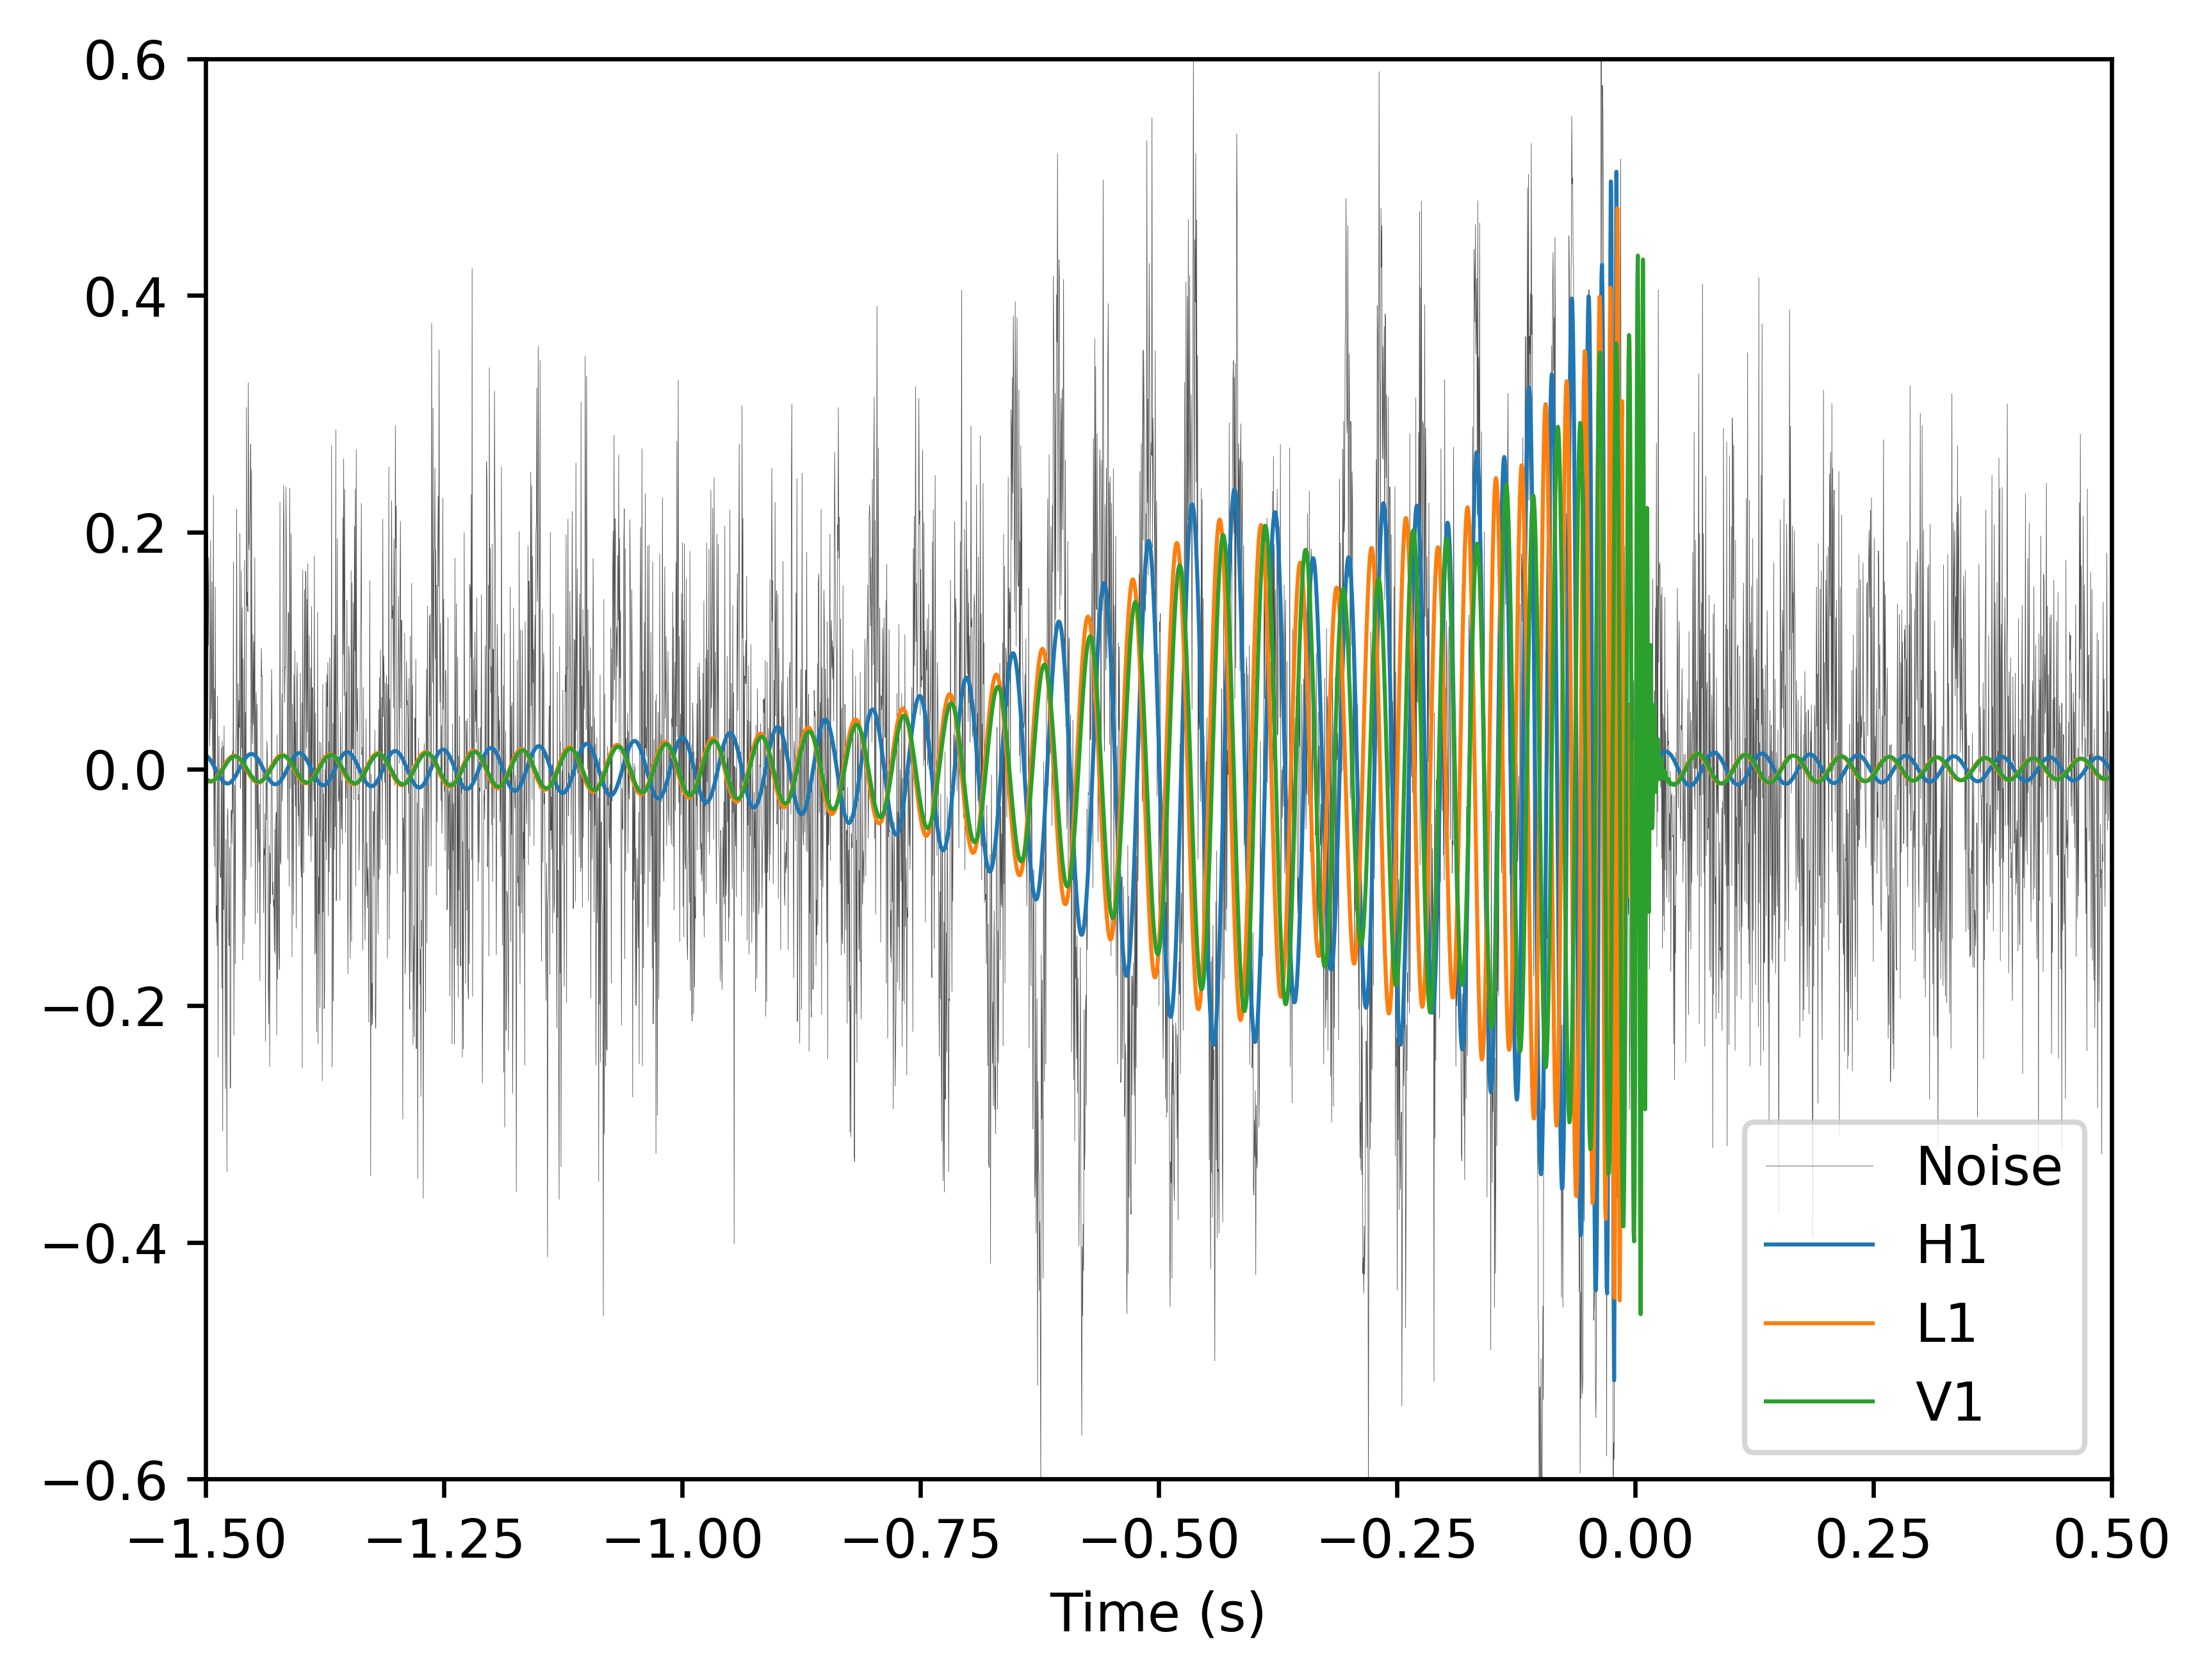
\includegraphics[width=1\linewidth]{media/images/obs_time_domain_lowSNR.png}
  \caption{Gravitational wave signal of the target observation $\boldsymbol{x}_0$ in the time domain, with and without noise added. Only 2\,s of the entire 4\,s signal is shown. The two black holes merge at the moment t=0s.}
  \Description[<short description>]{<long description>}
  \label{fig:obs_time_domain}
  \myvspacecommand
\end{figure}

\begin{figure}[tb]
  \centering
  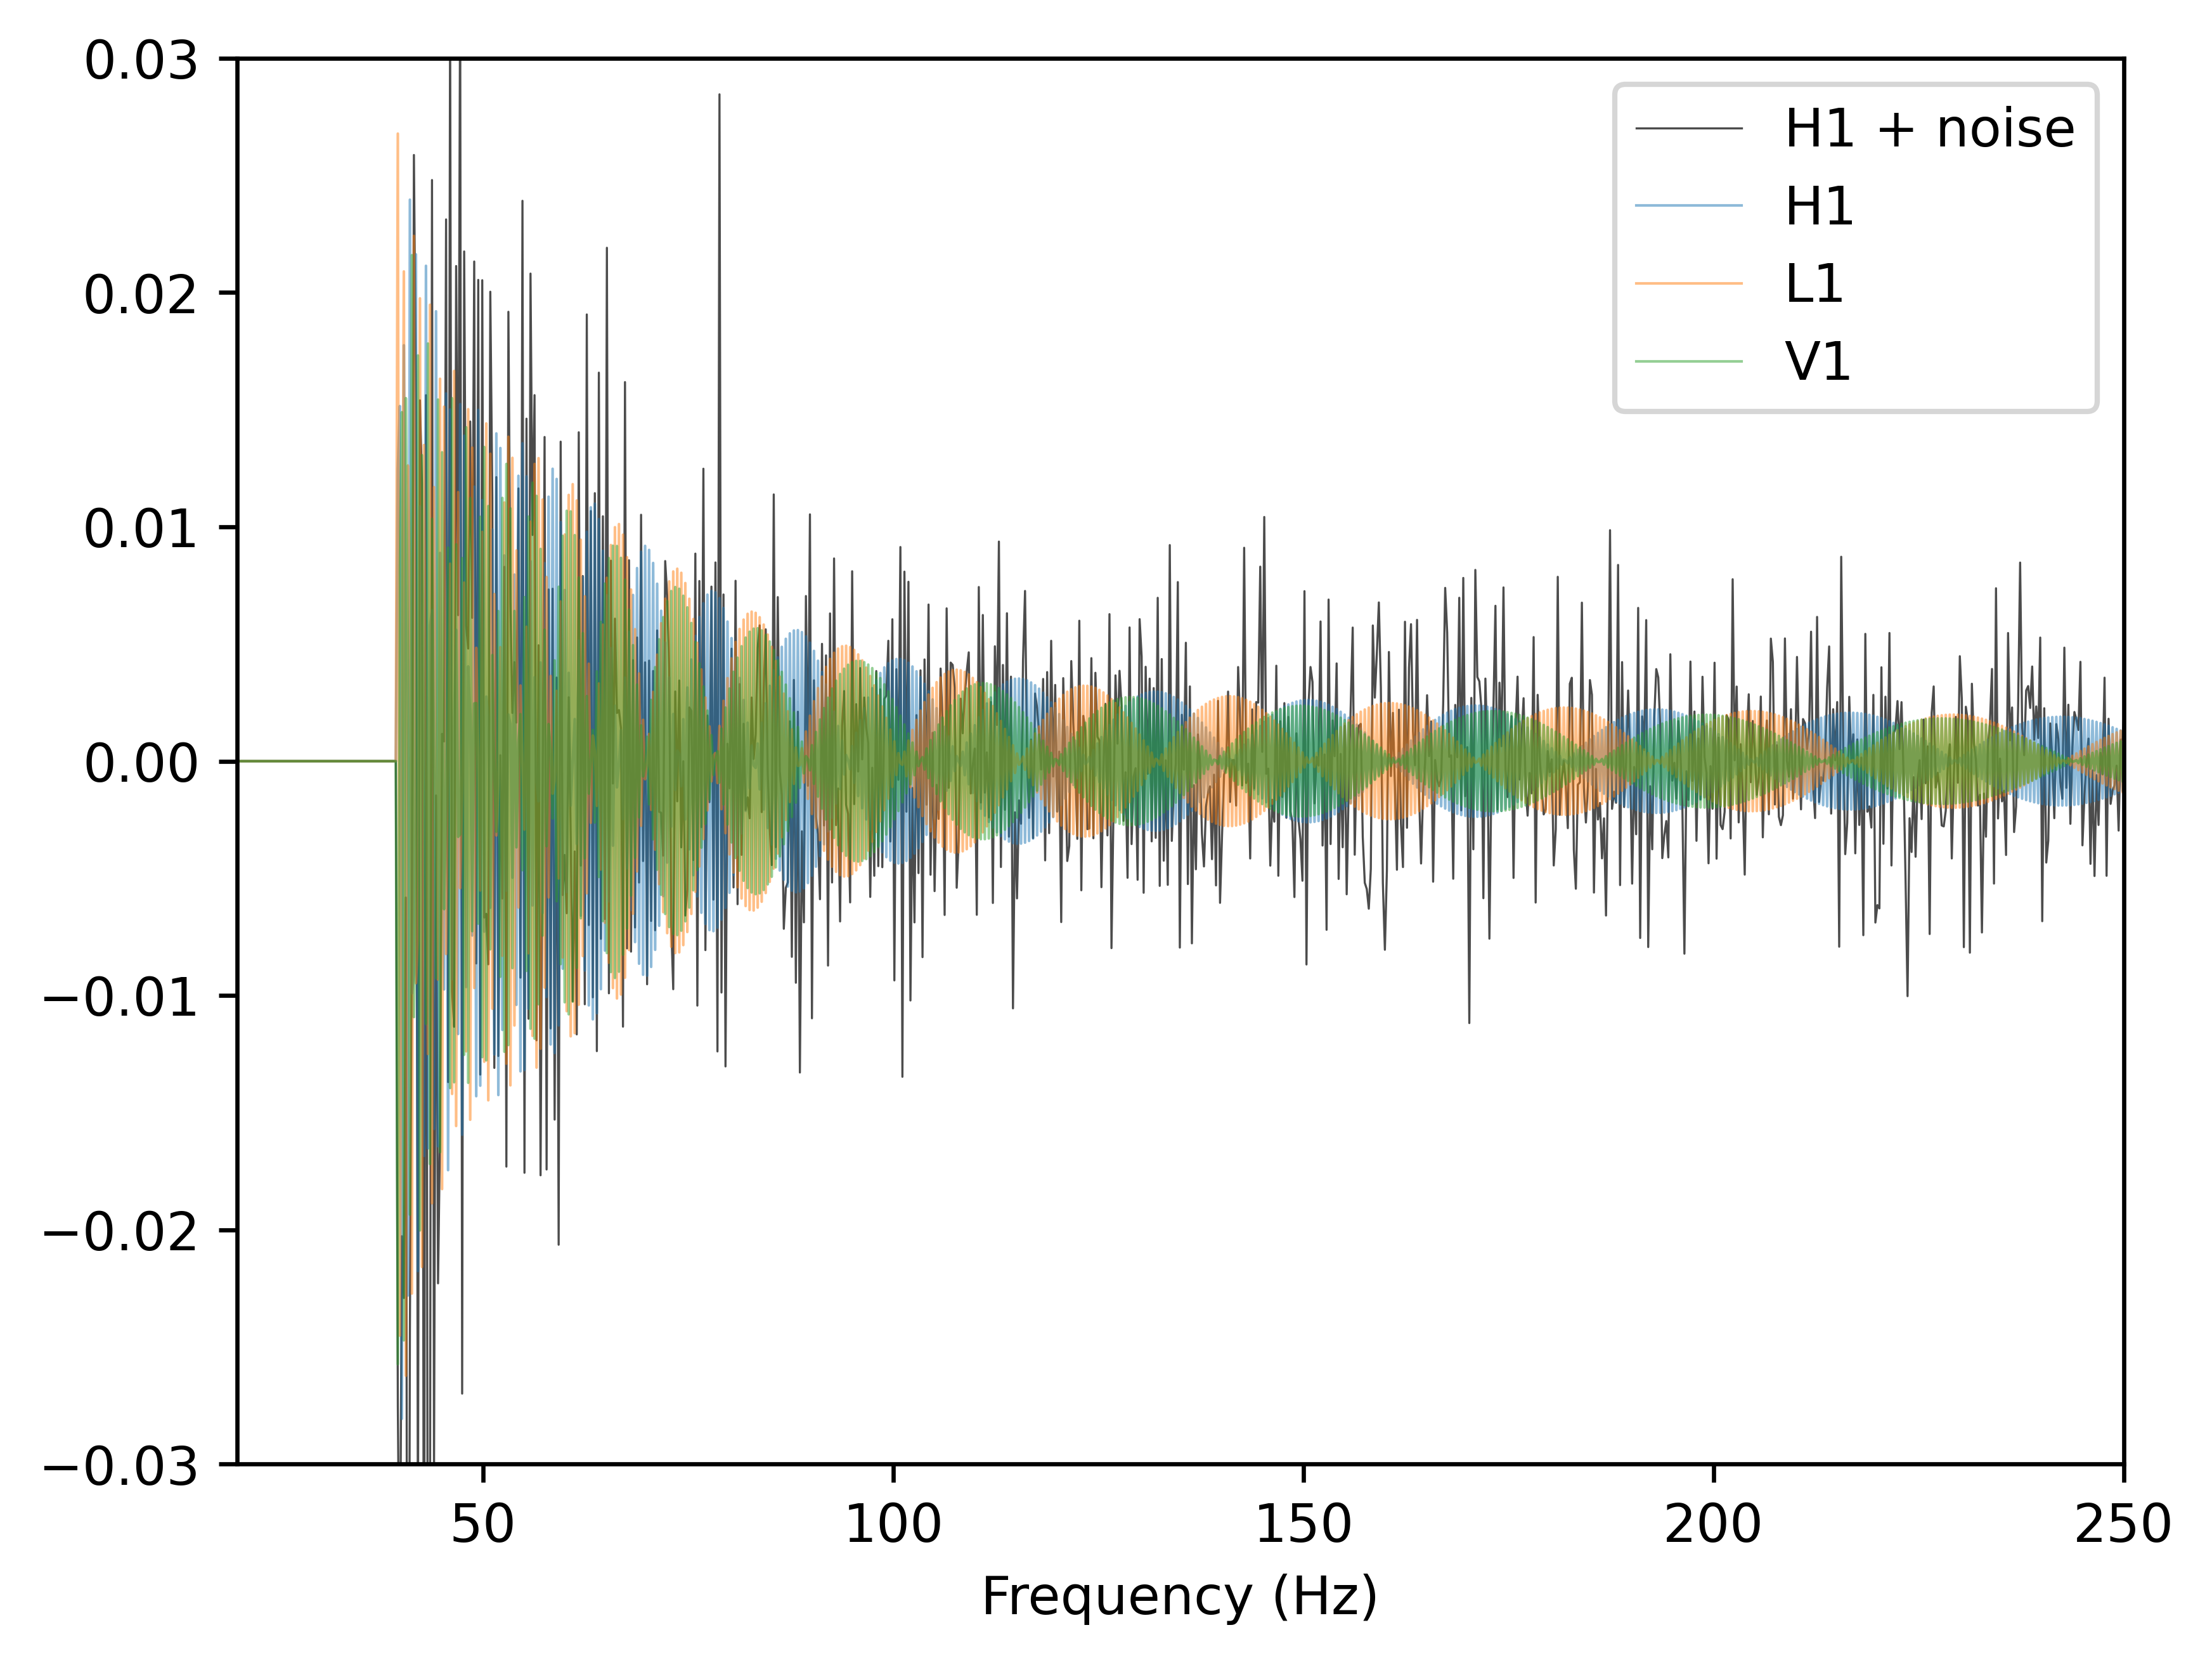
\includegraphics[width=1\linewidth]{media/images/obs_freq_domain_lowSNR.png}
  \caption{Gravitational wave signal of the target observation $\boldsymbol{x}_0$ in the frequency domain, with and without noise added. The full frequency range extends up to 1024\,Hz.}
  \Description[<short description>]{<long description>}
  \label{fig:obs_freq_domain}
  \myvspacecommand
\end{figure}

All of the waveform data used here was simulated (further details explained in section~\ref{sec:method_peregine_simulate}), since experimentally measured signals are rare (only 90 detections so far), which is insufficient data to train a neural network with. In the original \texttt{peregrine} paper, two example observations were used for the case studies - one with a high signal-to-noise ratio of $\sim$100, and another with low signal-to-noise ratio of $\sim$20. In this study, we will only consider the low signal-to-noise ratio example, since it is essential that the network can reliably distinguish signal from noise, and the high signal-to-noise ratio is a somewhat unphysical example~\cite{bhardwaj2023peregrine}.

The target observation, $\boldsymbol{x}_0$ was generated using the 15 parameter values given in Table~\ref{tab:gw_parameters}. Ten of these parameters represent intrinsic properties of the source e.g. the masses and spins of the two black holes, while five of these are extrinsic parameters e.g. the distance from the source and orientation in the sky with respect to the observations. Given the accuracy these waveforms can be simulated with, the `target observation' in theory could be substituted for a real detected observation. However, we are using simulated observations here so we have reliable `ground-truth' data to validate the overall method with. This target observation can be seen in Figures~\ref{fig:obs_time_domain} and~\ref{fig:obs_freq_domain}. The wave signal itself can be divided roughly into three segments which corresponds to different phases of the merging event -- inspiral, merger and ringdown phases~\cite{Pan_GW_2014}. Various parameters affect each of these phases differently~\cite{bhardwaj2023peregrine}.


\begin{table}[htb]
\centering
\caption{Description of the parameters that describe the gravitational waveforms. Values for the target observation $x_0$, and the range and distribution functions of the priors are also given.}
\label{tab:gw_parameters}
\begin{tabular}{lll} 
\toprule
\textbf{Parameters, $\boldsymbol{\theta}_{GW}$} & \textbf{Prior, $p(\boldsymbol{\theta}_{GW})$} & \textbf{Target, $x_0$} \\ 
\midrule
\textit{Intrinsic} & & \\ 
Mass ratio, \( q \) & \( U(0.125, 1) \) & 0.8858 \\ 
Chirp mass, \( M \) [\( M_{\odot} \)] & \( U(25, 100) \) & 32.14 \\ 
Inclination angle, \( \theta_{jn} \) [rad] & sin(0, \( \pi \)) & 0.4432 \\ 
Phase, \( \phi_c \) [rad] & \( U(0, 2\pi) \) & 5.089 \\ 
Tilt angle, \( \theta_1 \) [rad] & sin(0, \( \pi \)) & 1.497 \\ 
Tilt angle, \( \theta_2 \) [rad] & sin(0, \( \pi \)) & 1.102 \\ 
Spin, \( a_1 \) & \( U(0.05, 1) \) & 0.9702 \\ 
Spin, \( a_2 \) & \( U(0.05, 1) \) & 0.8118 \\ 
Spin angle, \( \phi_{12} \) [rad] & \( U(0, 2\pi) \) & 6.220 \\ 
Spin angle, \( \phi_{jl} \) [rad] & \( U(0, 2\pi) \) & 1.885 \\ 
\midrule
\textit{Extrinsic} & & \\ 
Luminosity Distance, \( d_L \) [Mpc] & \( U_{\text{vol}}(100, 2000) \) & 900 \\ 
Right ascension, \( \alpha \) [rad] & \( U(0, 2\pi) \) & 5.556 \\ 
Declination, \( \delta \) [rad] & cos(-\( \pi/2 \), \( \pi/2 \)) & 0.071 \\ 
Polarisation angle, \( \psi \) [rad] & \( U(0, \pi) \) & 1.100 \\ 
Merger time, \( t_c \) [GPS s] & \( U(-0.1, 0.1) \) & 0.000 \\ 
\bottomrule
\end{tabular}
\end{table}

% ============================================================================ %
% TMNRE
% ============================================================================ %

\subsection{TMNRE}
\label{sec:tmnre}

\texttt{Peregine} implements a specific type of Simulation-based inference algorithm, called TMNRE (Truncated Marginal Neural Ratio Estimation) for estimating the marginal posteriors of a \textit{specific} targeted observation~\cite{Miller_TMNRE_2021}. To do this, we apply Bayes' theorem:

\begin{equation*}
    p(\theta|x) = \frac{p(x|\theta) p(\theta)}{p(x)} = r(x|\theta) p(\theta)
\end{equation*}

Where $p(\theta|x)$ is the posterior of parameters $\theta$ given some observed or simulated data $x$, $p(x|\theta)$ is the likelihood of given data $x$ given input parameters $\theta$, $p(\theta)$ is the prior distribution of $\theta$, $p(x)$ is the Bayesian evidence of $x$ and $r(x|\theta)$ is the likelihood-to-evidence ratio. The power of SBI arises because with a forward generative model, $p(x,\theta)=p(\theta|x) p(\theta)$, we are able to sample implicitly from the (simulated) likelihood~\cite{Cranmer_SBI_2020}.

From Bayes theorem, there are three SBI approaches for estimating the posterior distributions given a forward generative model. They are Neural Posterior Estimation (NPE), Neural Likelihood Estimation (NLE) and finally, Neural Ratio Estimation (NRE). Training a network to learn the posteriors or likelihoods directly is an unsupervised learning problem, whereas learning the likelihood-to-evidence ratio, $r(x|\theta) = p(\theta|x) / p(x)$ is a simpler task as it can be translated into a supervised learning problem~\cite{Cranmer_SBI_2020}. In what is also known as the \textit{likelihood ratio trick}, a binary classifier can be trained to differentiate between jointly drawn $(x,\theta) \sim p(x,\theta)$ and marginally drawn samples $(x,\theta) \sim p(x)p(\theta)$~\cite{Brehmer_Cranmer_2020}. The output of this trained classifier $\hat{s}(x|\theta)$ can then be used as an estimator for the likelihood ratio, $\hat{r}(x|\theta)$,
\begin{equation*}
    \hat{r}(x|\theta) = \frac{1-\hat{s}(x|\theta)}{\hat{s}(x|\theta)}
\end{equation*}
This classifier is parameterized, and takes the parameters $\theta$ as explicit inputs. This means that for $k$ parameters, the network is training $k$ different binary classifiers simultaneously. Typically, the binary cross-entropy is used as a loss function, since this is most suited to multi-label binary classification tasks.

The likelihood-to-evidence ratio of a \textit{specific} target observation, $x_0$ is iteratively determined through several rounds of calculations. The posteriors of one round are used to truncate the boundaries of the prior distribution for the following round. This truncation serves to reduce the variance of the training samples each successive round, moving them closer to the target observation and allows for higher precision targeted inference. It is important to choose a conservative cut-off, since an over confident estimate risks reducing the parameter range too much. In \texttt{Peregrine}, this cut-off occurs where the posterior falls below $10^{-5} (4.26\sigma$ assuming a standard normal distribution). This targeted approach is much more simulation efficient, however it does lack the flexibility of a fully amortized approach~\cite{Miller_TMNRE_2021}.  

Only the marginal posteriors of each parameters are calculated, rather than the full joint posterior, since for many complex problems, extracting the full joint distributions is prohibitively expensive and for most scientific purposes the marginals are generally sufficient~\cite{Miller_TMNRE_2021}. 

% ============================================================================ %
% Peregrine
% ============================================================================ %

\subsection{Peregrine inference pipeline}
\label{sec:methodology_peregrine}

The \texttt{Peregrine} pipeline applies several sequential rounds of TMNRE to infer the posterior distributions of the 15 parameters of our target observation $\boldsymbol{x}_0$. An overview of a single round of the Peregrine inference pipeline is illustrated in Figure~\ref{fig:peregrine_pipeline}. The following section will go through the process and describe each of the steps in more detail.

\begin{figure}[htb]
    \centering
    \begin{tikzpicture}[node distance=2cm]
        \node (sampling) [sample] {\textbf{Sample} parameters $\boldsymbol{\theta}_{GW}$ from prior $p(\boldsymbol{\theta}_{GW})$};
        \node (fsimulator) [simulator, below of=sampling, yshift=0.1cm] {\textbf{Simulate} waveforms $\boldsymbol{x}(\theta_{GW}) = h(\theta_{GW}) + n_{IFO}$};
        \node (network) [network, below of=fsimulator, yshift=-0.05cm] {\textbf{Train} network to estimate likelihood-to-evidence ratios $r(\boldsymbol{x};\theta_k) = p(\theta_k|\boldsymbol{x})/p(\theta_k)$ for all parameters $k$};
        \node (inference) [inference, below of=network, yshift=0.2cm] {Bayesian \textbf{Inference}};
        \node (prior) [pinput, left of=inference, xshift=-0.8cm] {Prior samples from $p(\theta)$};
        \node (target) [tinput, right of=inference, xshift=0.8cm] {Target Observation $\boldsymbol{x}_0$};
        \node (ratios) [output, below of=inference, xshift=-0.0cm, yshift=0.4cm] {Ratios $r(\boldsymbol{x}_0;\theta)$};
        \node (posterior) [output, left of=ratios, xshift=-0.8cm] {Posteriors $p(\theta|\boldsymbol{x}_0)$};
        \draw [arrow] (sampling) -- node[anchor=west] {$\boldsymbol{\theta}_{GW}$} (fsimulator);
        \draw [arrow] (fsimulator) -- node[anchor=west] {$\boldsymbol{\theta}_{GW},\boldsymbol{x}$} (network);
        \draw [arrow] (network) -- (inference);
        \draw [arrow] (prior) -- (inference);
        \draw [arrow] (target) -- (inference);
        \draw [arrow] (inference) -- (ratios);
        \draw [arrow] (ratios) -- (posterior);
       % \draw [arrow] (prior) -- (posterior);
        \draw [arrow] (posterior) -- +(-1.5,0) |- node[anchor=west, yshift=-2cm, text width=2cm]{Using $p(\theta|\boldsymbol{x}_0)$ truncate prior $p(\boldsymbol{\theta}_{GW})$ and repeat rounds until converged} (sampling);
    \end{tikzpicture}
    \caption{High-level overview of the \texttt{peregrine} simulation-based inference method used for this work.}
    \Description[<short description>]{<long description>}
    \label{fig:peregrine_pipeline}
    \myvspacecommand
\end{figure}

\subsubsection{Sample Parameters} 

To begin, input parameters $\boldsymbol{\theta}_{GW}$ are randomly sampled from the prior distributions, $p(\theta_{GW})$. It is assumed that all parameters are independent i.e. not correlated with each other. The number of times we sample is determined by how many simulations, $N$ we wish to run in the next step.

\subsubsection{Simulate Waveforms}
\label{sec:method_peregine_simulate}
Given the $N$ values of $k=15$ input parameters, the data $x \sim p(x|\boldsymbol{\theta}_{GW}$) for training the network is simulated. The waveforms were simulated using the open source Bilby code~\cite{Ashton_Bilby_2019}, which is capable of generating theoretical predictions of GW signals based on several source models, waveform approximants, instrument noise and detector responses.

The sampling and simulations were controlled using the \texttt{Simulator} class which is part of the \texttt{swyft} library~\cite{Miller2022}. The GW waveform is simulated both in the time and frequency domain, including the detector noise. The signal and noise components of the signal remain separate for the time being.

\subsubsection{Train Network}

An overview of the network training step in \texttt{Peregrine} is given in Figure~\ref{fig:peregrine_network_step}. The network structure consists of two parallel U-Net networks, which process the time and frequency domain strains of the waveform independently. The noise of the signal is treated in the following way. Within each batch of samples fed to the network, the noise data is shuffled and randomly assigned to another sample in the same batch, where it is added to the signal. Therefore, for each epoch, the network sees training samples with the same signal component, but different noise component. This helps prevent the network over-fitting to the noise in the signal~\cite{bhardwaj2023peregrine}.

\begin{figure}[htb]
    \centering
    \begin{tikzpicture}[node distance=2cm]
			%%% NODES
			\node (dt) [per_input, label=west:\small 8192$\times$3] { $d(t)+n(t)$ };
			\node (df) [per_input, right of=dt, xshift=1cm, label=east:\small 4097$\times$6] {$\tilde{d}(f)+\tilde{n}(f)$};
			\node (unet_t) [per_unet, below of=dt, yshift=1cm, text width=2cm] { U-Net / Transformer };
			\node (unet_f) [per_unet, below of=df, yshift=1cm, text width=2cm] { U-Net / Transformer };
			\node (feature_t) [per_features, below of=unet_t, label=west:\small 16$\times$1, yshift=1cm] { $t$ summary stats };	
			\node (feature_f) [per_features, below of=unet_f, label=east:\small 16$\times$1, yshift=1cm] { $f$ summary stats };
			\node (concat) [per_concat, below of=feature_t, xshift=1.5cm, label=east:\small 32$\times$1, yshift=1cm] { Concatenate };
			\node (MLP) [per_MLP, below of=concat, yshift=1cm] { MLP (swyft) };
			\node (labels) [per_labels, right of=MLP, xshift=0.5cm, text width=1.0cm] { $\theta_{GW}$ labels };
			\node (lograts) [per_logratios, below of=MLP, label=east:\small 15$\times$1, yshift=1cm] { Logratios };
			%%% EDGES			
			\draw [arrow_unet] (dt) -- node[anchor=west]{}(unet_t);
			\draw [arrow_unet] (df) -- node[anchor=west]{}(unet_f);
			\draw [arrow_unet] (unet_t) -- node[anchor=west]{}(feature_t);
			\draw [arrow_unet] (unet_f) -- node[anchor=west]{}(feature_f);
			\draw [arrow_unet] (feature_t) -- node[anchor=west]{}(concat);
			\draw [arrow_unet] (feature_f) -- node[anchor=west]{}(concat);
			\draw [arrow_unet] (concat) -- node[anchor=west]{}(MLP);
			\draw [arrow_unet] (labels) -- node[anchor=west]{}(MLP);
			\draw [arrow_unet] (MLP) -- node[anchor=west]{}(lograts);
    \end{tikzpicture}
    \caption{Details of the neural network step in Peregrine. The numbers outside the boxes represent the output size of each step. Details of the U-Net architecture are given in Figure~\ref{fig:Attention_UNet_arch} in Appendix~\ref{sec:apx:u-net_architecture}.}
    \Description[<short description>]{<long description>}
    \label{fig:peregrine_network_step}
    \myvspacecommand
\end{figure}

The joint and marginal pairs of samples are created within each batch. Joint samples have the correct labels ($\theta_{GW}$) and are assigned to class 1, while the marginal samples have labels from a random sample within the same batch and are assigned to class 0. In essence, the network is trained to answer the question: \textit{Does this label belong to this sample? Yes/No?}. The loss function is the minimum of the total binary cross-entropy, i.e. the sum of the binary cross-entropy values over all parameters

The network outputs a vector of 16 features, or summary statistics, which ideally should capture all the relevant information from the waveform, in a low dimensional form. It is analogous to the class labels in a multi-class classification problem, but the classes in this case are learnt in an unsupervised way. The summary statistics from both the time and frequency domains are concatenated together before being passed to a simple multi-layer perceptron (MLP) which performs the final ratio estimation. This MLP is the default implemented in \texttt{swyft}.

The network architecture of the U-Net can be modified, or replaced entirely, while keeping the rest of the pipeline intact. The network determines the speed and quality of the summary statistics. The complete architecture of the (Attention) U-Net, as implemented in \texttt{peregrine} is given in Figure~\ref{fig:Attention_UNet_arch} (Appendix~\ref{sec:apx:u-net_architecture}).

The hyperparameters and TMNRE settings chosen are given in Table~\ref{tab:default_run_settings}. These settings are based on those in ~\cite{bhardwaj2023peregrine}, to ensure consistency and fair comparison to the baseline when comparing network modifications. The early stopping criteria terminates training if the validation loss has not decreased after the specified number of epochs. It could of course also be possible to try optimise these parameters further, however the focus of this work wanted to remain on the network architecture itself. The one exception is \enquote{simulations per round}, where we also ran a test case with half the number of simulations.



\begin{table}
    \centering
    \caption{\texttt{Peregrine} network hyperparameter and TMNRE settings.}
    \label{tab:default_run_settings}
    \begin{tabular}{ll}
         \toprule
         \textbf{Setting}  & 
         \textbf{Value} \\
         \midrule
         \textit{Network} & \\
         Min. epochs & 30 \\
         Max. epochs & 200 \\
         Early stopping & 7 \\
         Optimiser & Adam \\
         Learning rate & $5\times10^{-4}$\\
         Learning rate decay & Patience 5, factor 0.3\\
         Batch size & 256\\
         Train : val split & 0.9 : 0.1\\
         \midrule
         \textit{TMNRE} & \\
         Number of rounds & 8 \\
         Simulations per round & \multicolumn{1}{p{4cm}}{\raggedright 30k, 60k, 90k, 120k, 120k, 150k, 150k, 150k} \\
         \bottomrule
    \end{tabular}
    \myvspacecommand
\end{table}

\subsubsection{Inference}

After the training step is complete, an inference step is performed. Here, we use the trained network to determine the likelihood-to-evidence ratios for each of the parameters in the target observation. 
Then we can construct histograms of the posteriors by sampling from the prior $\theta \sim p(\theta)$, and weighting each prior sample with the likelihood-to-evidence ratio $\hat{r}(x_0|\theta)$~\cite{Miller_TMNRE_2021}.

At the end of each round, we truncate the priors for the subsequent round if the posterior probability is incredibly low i.e. $\epsilon$ less than 1e-5 ($\sim4.62\sigma$). This reduces the variance of the training data for the following round, edging it closer to more resemble the target observation, and thus allowing us to increase the precision of the inference. The algorithm is considered converged after a number of rounds once the truncation has finished and the posterior distributions stabilised.

% ============================================================================ %
% Attention U-Net
% ============================================================================ %
\subsection{Attention U-Net}

The U-Net architecture was modified with an additive attention gate as introduced in~\cite{Oktay_2018_AUNet}. In U-Net, there are skip connections that concatenate the feature maps from the encoder with the matching feature map of the decoder. The attention gate filters the encoder features by scaling with learned attention coefficients which suppresses irrelevant features (see Figure~\ref{fig:Attention_UNet_arch}). The output of the attention gate is element wise multiplication of the encoder feature map by the attention coefficients.

A schematic diagram of the attention gate added to the U-Net architecture in \texttt{Peregrine} is shown in Figure~\ref{fig:attention_gate}. To get to the attention coefficients,  the encoder part, $g$ and decoder part, $x$ pass a convolution of kernel size 1 
before being summed together, followed by a ReLU activation function. This is passed to another convolution with kernel size 1 and a single output channel, followed by a sigmoid activation function. The sigmoid function outputs the attention coefficients,  $\alpha$ which have a value between 0 and 1. The major difference between this attention gate, and that proposed in~\cite{Oktay_2018_AUNet}, is that there is no resampler directly after the sigmoid layer. This is because the U-Net in \texttt{Peregrine} does not upsample the features, but rather does zero-padding instead.

\begin{figure}[htb]
\centering
\begin{tikzpicture}[node distance=1.0cm]
    %%% NODES
    \node (wg) [wg] { $W_g : 1\times1$ };
    \node (wx) [wx, below of=wg] { $W_x : 1\times1$ };
    \node (plus) [plus, right of=wg, xshift=0.25cm, yshift=-0.5cm, label={[scale=2.0]center:$+$}] {};
    \node (relu) [relu, right of=plus, xshift=0.15cm] {ReLU};
    \node (psi) [psi, right of=relu, xshift=0.5cm] {$\psi: 1\times1$};
    \node (sigmoid) [sigmoid, right of=psi, xshift=0.35cm] {$\sigma$};
    \node (times) [times, right of=sigmoid, label={[scale=2.0]center:$\times$}, xshift=0.1cm] {};
    %%% EDGES			
    \draw [arrow_unet] (wg) -| node[anchor=west]{}(plus);
    \draw [arrow_unet] (wx) -| node[anchor=west]{}(plus);
    \draw [arrow_unet] (plus) -- node[anchor=west]{}(relu);
    \draw [arrow_unet] (relu) -- node[anchor=west]{}(psi);
    \draw [arrow_unet] (psi) -- node[anchor=west]{}(sigmoid);
    \draw [arrow_unet] (sigmoid) -- node[anchor=south]{$\alpha$}(times);
    \draw [arrow_unet] (wg.west) +(-0.7cm,0) -- node[anchor=south]{$g$}(wg.west);
    \draw [arrow_unet] (wx.west) +(-0.7cm,0) -- node[anchor=south]{$x$}(wx.west);
    \draw [arrow_unet] (times.east)  (times.east) -- node[anchor=south]{$x'$}+(0.5cm,0);
    \draw [arrow_unet] (wx.west) +(-0.35cm,0) -- +(-0.35cm,-0.7cm) -| (times.south);
\end{tikzpicture}
\caption{Schematic of the attention gate added to the U-Net architecture. $g$ refers to the encoder part passed through the skip connection, and $x$ refers to the decoder part. Adapted from~\cite{Oktay_2018_AUNet}.}
\Description[<short description>]{<long description>}
\label{fig:attention_gate}
\myvspacecommand
\end{figure}

% ============================================================================ %
% Transformer models
% ============================================================================ %
\subsection{Transformer models}

Two transformer architectures were tested, the 1D Vision transformer (ViT)~\cite{Dosovitskiy_2021_ViT}, and a transformer model specifically designed for multi-variate time series (MTS)~\cite{Zerveas_2020_mvts}. As a starting point, both models were taken and adapted from open-source GitHub repositories\footnote{MTS: \url{https://github.com/gzerveas/mvts_transformer/blob/master/src/models/ts_transformer.py}\\
ViT: \url{https://github.com/lucidrains/vit-pytorch/blob/main/vit_pytorch/vit_1d.py}}. Figure~\ref{fig:peregrine_network_step} indicates how the transformer models were placed within \texttt{Peregrine}. The models consisted of only the encoder part of the transformers, where they were trained to construct the summary statistics for both the time and frequency domains. The rest of the \texttt{peregrine} pipeline proceeded as normal. 

The original MTS model was adapted because the maximum batch size could only be 1-2 samples before the 40\,GB memory of a single A100 GPU was exceeded. Batch sizes cannot be this small because we need to randomly shuffle labels and noise within the batches for effective training. Memory requirements of transformers scale quadratically with sequence length, since self-attention scores are calculated for all possible pairs of input tokens in a given sequence. In the MTS model, each token is assumed to be a data point, and due to the size of the input data here, the memory requirements became prohibitive. To deal with this limitation, we incorporated the linear patching step from the ViT model into the MTS model.

\subsubsection{Hyperparameter tuning}

Transformer models contain numerous hyperparameters that can significantly impact their performance. The objective of the hyperparameter tuning was to find the best performing model within a limit of 10-20 epochs (30\,000 training samples per epoch). It was important for us to optimise to not only the loss function, but also the computation time as well. The training samples were generated from the full prior distributions (Table~\ref{tab:gw_parameters}). 

To find the optimal hyperparameters for each of the two models, we used the Python library Ray Tune~\cite{liaw2018tune} in combination with the Hyperopt \enquote{Tree-structured Parzen Estimator} (TPE) search algorithm~\cite{Bergstra_Bardenet_Bengio_Kégl_2011}. Ray Tune provides the framework to explore the hyperparameter space in an efficient way, due to early-stopping of unpromising trials which leaves more computational budget for the most promising trials. The TPE search algorithm is a Bayesian optimization method that takes into account performance of previous hyperparameters to make informed choices about the hyperparameters in following trials.

The options and chosen values for the hyperparameters for both the ViT and MTS transformer models are shown in Table~\ref{tab:transformer_hyperparams}. Full details regarding the hyperparameter tuning trials is given in Appendix~\ref{sec:apx:Hyperparameter_tuning}.

\begin{table}[htb]
    \centering
    \caption{Hyperparameter choices for the transformer models. The selected options are shown in bold.}
    \label{tab:transformer_hyperparams}
    \begin{tabular}{lll}
    \toprule
    \textbf{Hyperparameter} & \textbf{ViT values} & \textbf{MTS values} \\ 
    \midrule
    Batch size           & 16, 32, \textbf{64}, 128 & 16, \textbf{32}, 64 \\
    Learning rate        & 1e-5 -- 1e-3 (\textbf{1.6e-4}) & 1e-5 -- 1e-3 (\textbf{1e-4}) \\
    Patch size           & 4, 8, \textbf{16}, 32 & \textbf{16} \\
    Classes              & \textbf{16}, 24, 32 & \textbf{16} \\
    Dim embeddings       & 256, \textbf{512}, 1024 & \textbf{128}, 256, 512 \\
    Layers               & 4--10 (\textbf{7}) & 3--8 (\textbf{6}) \\
    Attention heads      & 4--10 (\textbf{6}) & \textbf{4}, 8, 16 \\
    Dim MLP              & \textbf{1024}, 2048 & 256, 512, \textbf{1024} \\
    Dropout              & \textbf{0}, 0.05, 0.1 & \textbf{0}, 0.05, 0.1 \\
    Embed dropout        & \textbf{0}, 0.05, 0.1 & - \\
    Position encoding    & - & \textbf{Fixed}, learnable \\
    \bottomrule
    \end{tabular}
    \myvspacecommand
\end{table}

A schematic diagram of the ViT architecture, reproduced from~\cite{Vaswani_2017_transformer}, is given in Figure~\ref{fig:vit_model_architecure} to help explain the different hyperparameters. The transformer encoder block consists of several alternating layers of a multi-head self-attention mechanism and an inner feed-forward network (MLP). The feed-forward network has two layers with a GeLU non-linear activation function. The dropout serves as a regularization parameter by randomly dropping a fraction of the connections between nodes in the network.

\begin{figure}[htb]
  \centering
  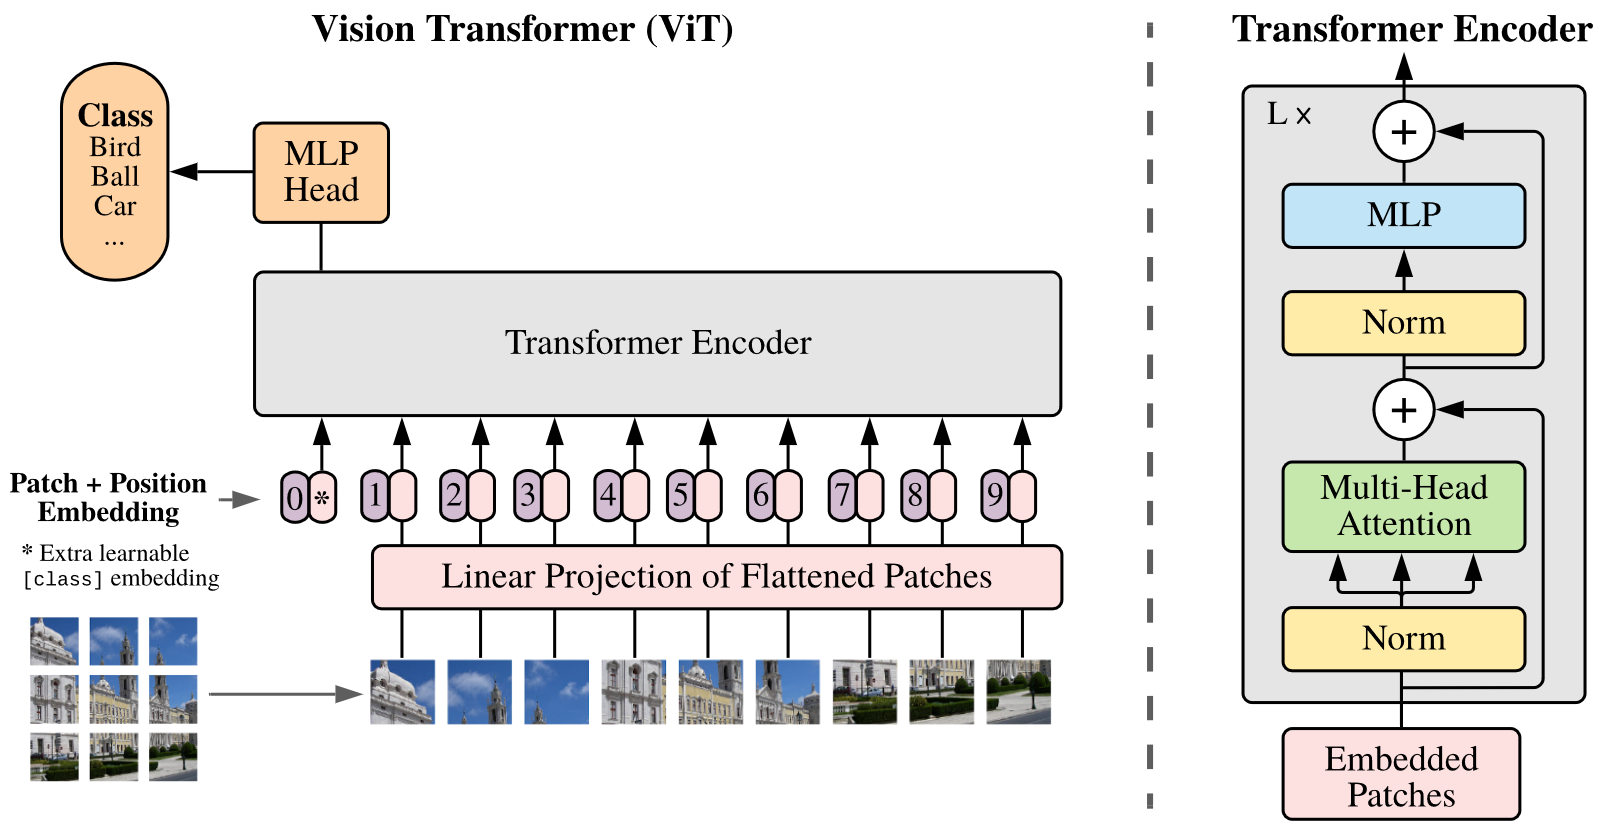
\includegraphics[width=1\linewidth]{media/images/ViTmodel.PNG}
  \caption{Schematic overview of the original ViT model. Reproduced from~\cite{Vaswani_2017_transformer}.}
  \Description[<short description>]{<long description>}
  \label{fig:vit_model_architecure}
  \myvspacecommand
\end{figure}

\subsubsection{Pretraining}

Before introducing into \texttt{peregrine}, both transformer models were pretrained for 24 hours with single A100 GPU on 2 million generated waveforms ($\sim$750\,GB). For comparison purposes, the original U-Net model also underwent the same pretraining procedure. Regular validation checks were performed to track the performance and ensure no overfitting occurred. The validation split of the data was 95\% for training and 5\% for validation checks. The saved weights from pretraining were used to initialise the network during each \texttt{peregrine} run. 

% ============================================================================ %
% Pruning
% ============================================================================ %
\subsection{Pruning}

The U-Net models for the time and frequency domain were pruned individually, using the DepGraph \enquote{torch\_pruning} library~\cite{Fang_Ma_Song_Mi_Wang_2023} with the trained U-Net model from the pre-training process as input. Two pruned models were created, one that had 5\% of channels removed, and another with 10\% removed.


% ============================================================================ %
% Evaluation
% ============================================================================ %
\subsection{Evaluation}

The current Peregrine pipeline requires 8 rounds of sequential TMNRE, 720000 simulated waveforms and around 12.5 hours (on a single A100 GPU with 18 CPU cores) to completely reconstruct the posteriors of the fifteen parameters to their statistical limit. Of these 12.5 hours, around 10 is for training the network and 2.3 is for simulating the waveforms used for training the network. 

To compare the performance of the different networks, a suitable metric needs to be chosen. For a binary classifier, the AUROC (Area Under the Receiver Operating Characteristic) curve is a single scalar value that effectively describes the performance of the network over all possible thresholds. A value of 0.5 is a random classifier, while a value of 1 is a perfect classifier. Values between 0.5 and 1 suggest the network has some ability to distinguish between the two classes. We have calculated the AUROC for each parameter, as well as the average over all 15 parameters by applying a softmax function to the raw logits to get the probabilities, before feeding into sklearn's \enquote{roc\_auc\_score} function.

Although the AUROC is a simple metric to quantify the performance of the binary classifier, it is not enough in this case. This is because the network trains over several rounds, and the variance of the samples reduces each round. Therefore, in later rounds,  the waveforms become more similar and it becomes more challenging for the network to differentiate between the two classes. Some networks may perform well in the early rounds, but then later on perform poorly. We thus introduce an additional metric, the \enquote{truncation fraction}, which quantifies the fraction of the sampling volume (15D) remaining after truncating the prior distributions at the end of each round. It is a way to measure how effectively the network is able to \enquote{zoom-in} to the parameter range of interest.

The results of the original \texttt{peregrine} have themselves been benchmarked against established likelihood-based methods~\cite{Speagle_2020}, and found to be in good agreement. Therefore, in this work we think it is sufficient to compare only with the original \texttt{peregrine}.

%\todo[inline]{Number of trainable parameters}

%The architecture of the network currently implemented in \texttt{peregrine} is the U-Net architecture~\cite{Ronneberger_UNet_2015}. Given the advances in machine learning and CNN architectures since 2015, it is believed that this network can be improved upon. The optimisation of this network architecture will be the main focus of this thesis. 

%Investigative studies will be performed to find the best network architectures most suitable for the data format. We will first try with LSTM's since they are known to work well with noisy time-series data. The chosen network architecture also needs to be capable of segmenting the signal into three components, representing the different stages of the merger event -- inspiral, merger and ringdown~\cite{Pan_GW_2014}. Each of the parameters in $\boldsymbol{\theta}_{GW}$ are impacted differently in the different phases~\cite{bhardwaj2023peregrine}. Given the network is a binary classifier that classifies between joint and marginally drawn sample pairs, we will assess the performance of the network with the ROC curve.